\documentclass[a4paper,12pt]{article}
\usepackage{amsmath}
\interdisplaylinepenalty=200
\usepackage{amsthm}
\usepackage{amssymb}
\usepackage[dvips]{graphicx}
\usepackage[OT4]{fontenc}
\usepackage[utf8]{inputenc}
\usepackage{xcolor}
\usepackage{pgf}
%\usepackage{tikz}
%\usetikzlibrary{shapes,arrows,positioning}
\usepackage{url}
\usepackage{calc}
\usepackage{cancel}
\usepackage{bm}
\usepackage{setspace}
%\usepackage{logoipi}
%\usepackage[round]{natbib}
\usepackage[square,numbers]{natbib}
%\usepackage[round]{natbib}
% \usepackage[unicode,debug,colorlinks=true,linkcolor=red,citecolor=red,urlcolor=red,pdfusetitle=true,breaklinks=true]{hyperref}
\usepackage[unicode,debug,colorlinks=true,linkcolor=black,citecolor=black,urlcolor=black,pdfusetitle=true,breaklinks=true]{hyperref}
%\usepackage{makeidx}
\emergencystretch=20pt

%\renewcommand{\bibsection}{\chapter*{\bibname}}
\newcommand{\bibnamefont}[1]{\MakeUppercase{#1}}
\newcommand{\toprule}{\hline}
\newcommand{\midrule}{\hline}
\newcommand{\botrule}{\hline}
\bibliographystyle{abbrvnat}

\newcommand{\abs}[1]{\left| #1 \right|}
\newcommand{\norm}[1]{\left|| #1 \right||}
\newcommand{\okra}[1]{\left( #1 \right)}
%\newcommand{\join}[1]{\left( #1 \right)}
\newcommand{\join}[1]{\left\langle #1 \right\rangle}
%\newcommand{\mean}[1]{\textbf{E}\kwad{#1}}
\newcommand{\mean}[1]{\mathbf{E}\, #1}
\newcommand{\ceil}[1]{\left\lceil #1 \right\rceil}
\newcommand{\floor}[1]{\left\lfloor #1 \right\rfloor}
\newcommand{\kwad}[1]{\left[ #1 \right]}
\newcommand{\klam}[1]{\left\{ #1 \right\}}
\newcommand{\subst}[1]{\left. #1 \right|}
%\newcommand{\ind}{\mathrel{\perp\mkern-10mu\perp}}
%\newcommand{\norm}[1]{\left|\mkern-1mu\left| #1 \right|\mkern-1mu\right|}
\newcommand{\boole}[1]{{\bf 1}{\klam{#1}}}
%\DeclareMathOperator{\essinf}{ess\,inf}
\DeclareMathOperator{\re}{Re}
\DeclareMathOperator{\im}{Im}
\DeclareMathOperator{\const}{const}
\DeclareMathOperator{\erf}{erf}
\DeclareMathOperator{\Li}{Li}
\DeclareMathOperator{\card}{card}
\DeclareMathOperator{\cov}{Cov}
\DeclareMathOperator{\var}{Var}
\DeclareMathOperator{\corr}{Corr}
\DeclareMathOperator*{\argmax}{arg\,max}
\DeclareMathOperator*{\argmin}{arg\,min}
\newcommand{\peq}{\stackrel{+}{=}}
\newcommand{\pge}{\stackrel{+}{>}}
\newcommand{\ple}{\stackrel{+}{<}}
\newcommand{\meq}{\stackrel{*}{=}}
\newcommand{\mge}{\stackrel{*}{>}}
\newcommand{\mle}{\stackrel{*}{<}}

\title{The Supplementary Materials for Article ``Corrections of Zipf's
  and Heaps' Laws Derived from Hapax Rate Models''}

\author{{\L}ukasz D\k{e}bowski%
  \thanks{{\L}. D\k{e}bowski is with the Institute of Computer
    Science, Polish Academy of Sciences, ul.\ Jana Kazimierza 5,
    01-248 Warszawa, Poland (e-mail: ldebowsk@ipipan.waw.pl).}}
\date{}

\begin{document}
%\layout
\maketitle

% \begin{abstract}
%   This is the supplementary report for article ``Corrections of Zipf's
%   and Heaps' Laws Derived from Hapax Rate Models''. The article
%   introduces corrections to Zipf's and Heaps' laws based on systematic
%   models of the hapax rate. The derivation rests on two assumptions:
%   The first one is the standard urn model which predicts that marginal
%   frequency distributions for shorter texts look as if word tokens
%   were sampled blindly from a given longer text. The second assumption
%   posits that the rate of hapaxes is a simple function of the text
%   size. Four such functions are discussed: the constant model, the
%   cancelation model, the linear model, and the logistic model. It is shown
%   that the logistic model yields the best fit. This report contains
%   all tables, all plots, and an instruction for rerunning the
%   numerical experiment.
%   \\[1ex]
%   \textbf{Keywords:} calculus, hapax rate, Heaps' law, urn model, Zipf's law
% \end{abstract}

\section{Introduction}
\label{secIntroduction}

This is the supplementary report for article ``Corrections of Zipf's
and Heaps' Laws Derived from Hapax Rate Models''. The article
introduces corrections to Zipf's and Heaps' laws based on systematic
models of the hapax rate. The derivation rests on two assumptions: The
first one is the standard urn model which predicts that marginal
frequency distributions for shorter texts look as if word tokens were
sampled blindly from a given longer text. The second assumption posits
that the rate of hapaxes is a simple function of the text size. Four
such functions are discussed: the constant model, the cancelation model, the
linear model, and the logistic model.  This report contains all
tables, all plots, and an instruction for rerunning the numerical
experiment.

\section{Running the experiment}

We worked on Linux Ubuntu 20.04.4 LTS applying a mixture of Bash,
Perl, and Gnuplot scripts.  We processed 14 texts in English
downloaded from Project Gutenberg \citep{Gutenberg11} and listed in
Table \ref{tabTexts}. These texts were projected to 26 letters and a
space (27 distinct characters in total), compressed by \verb}gzip},
and placed into directory \verb}gutenberg/}.  The scripts for running
the experiment are located in directories \verb}scripts/} and
\verb}TypeToken/}. To repeat the experiment, it suffices to run:
\begin{verbatim}
cd ./scripts/
./make.bash
\end{verbatim}
Script \verb}make.bash} calls other scripts in directories
\verb}scripts/} and \verb}TypeToken/}, which apply Bash, Perl, and
Gnuplot. Prior to running the experiment, make sure that you have
installed these in your operating system.  In particular, the final
Latex arrays for Tables \ref{tabPars} and \ref{tabWSSRs} are produced
by scripts
\begin{verbatim}
make_parameters_herdan_1.pl,
make_parameters_herdan_2.pl.
\end{verbatim}

\begin{table}[t]
\caption{The selection of texts from Project
  Gutenberg.\label{tabTexts}}
\centering
\medskip
\begin{tabular}{|l|l|r|}
  \toprule
  Title &Author &File \\
  \midrule
  First Folio/35 Plays &W. Shakespeare & {00ws110.txt} \\
  One of Ours&W. Cather & {1ours10.txt} \\
  20,000 Leagues under the &J. Verne & {2000010.txt} \\
  \hfill Sea & & \\
  Critical \& Historical Essays &T. Macaulay & {2cahe10.txt} \\
  Five Weeks in a Balloon &J. Verne & {5wiab10.txt} \\
  Eight Hundred Leagues on &J. Verne & {800lg10.txt} \\
  \hfill the Amazon & & \\
  The Complete Memoirs &J. Casanova & {csnva10.txt} \\
  Memoirs &Comtesse du Barry & {dbrry10.txt} \\
  The Descent of Man &C. Darwin & {dscmn10.txt} \\
  Gulliver's Travels &J. Swift & {gltrv10.txt} \\
  The Mysterious Island &J. Verne & {milnd10.txt} \\
  Mark Twain, A Biography &A. Paine & {mt7bg10.txt} \\
  The Journal to Stella &J. Swift & {stlla10.txt} \\
  Life of William Carey &G. Smith & {wmcry10.txt} \\
  \botrule
\end{tabular}  
\end{table}

\begin{figure}[t]
  \centering
  %\vspace{-4em}
  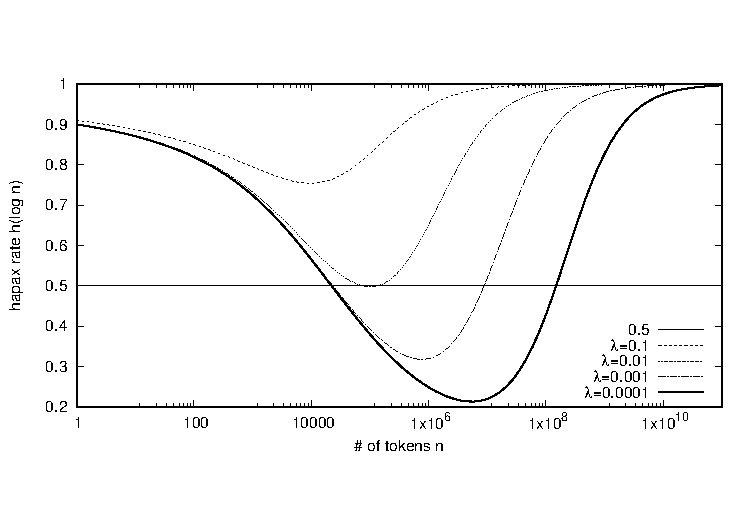
\includegraphics[width=\columnwidth]{output/token_ratio.pdf}
  %\vspace{-4em}
  \caption{The $U$-shaped hapax rate function for a mixture of the
    cancelation model with $\alpha=10$ and the maximal model. The weight of
    the cancelation model is $(1-\lambda)$ and the weight of the maximal
    model is $\lambda$. \label{figHapaxU}}
\end{figure}

\begin{table*}[p]
  \caption{The parameters fitted by least squares to function
    $G(n)$.\label{tabPars}}
  \centering
  \medskip
  \footnotesize
  \begin{tabular}{|l|l|l|lll|ll|r|}
    \toprule
    File & Constant & Cancelation
    & \multicolumn{3}{c|}{Logistic}
    & \multicolumn{2}{c|}{Linear} & Length\\
    \cline{2-2}\cline{3-3}\cline{4-6}\cline{7-8}
    & $\beta$       & $\alpha$
    & $\gamma$      & $\beta$       & $\alpha$
    & $\gamma$      & $\alpha$      & $N$\\
\midrule
00ws110.txt     & 0.768 & 12.06 & 0.314 & 0.218 & 10.11 & 0.0509        & 2.14  & 835726\\
1ours10.txt     & 0.797 & 11.55 & 0.318 & 0.203 & 9.72  & 0.0507        & 1.7   & 128963\\
2000010.txt     & 0.801 & 11.48 & 0.323 & 0.008 & 10.62 & 0.0578        & 2.22  & 101247\\
2cahe10.txt     & 0.796 & 12.12 & 0.314 & 0     & 11.38 & 0.0576        & 2.79  & 298339\\
5wiab10.txt     & 0.808 & 11.64 & 0.315 & 0.001 & 10.86 & 0.0552        & 2.13  & 92558\\
800lg10.txt     & 0.799 & 11.43 & 0.327 & 0.162 & 9.77  & 0.0534        & 1.84  & 95493\\
csnva10.txt     & 0.732 & 11.39 & 0.308 & 0.157 & 9.94  & 0.0542        & 1.87  & 1268149\\
dbrry10.txt     & 0.787 & 11.39 & 0.325 & 0.065 & 10.31 & 0.0583        & 2.23  & 159710\\
dscmn10.txt     & 0.774 & 11.5  & 0.328 & 0     & 10.75 & 0.0629        & 2.71  & 312075\\
gltrv10.txt     & 0.796 & 11.4  & 0.322 & 0.001 & 10.62 & 0.0584        & 2.22  & 104909\\
milnd10.txt     & 0.773 & 11.14 & 0.347 & 0.127 & 9.63  & 0.0608        & 2.24  & 195064\\
mt7bg10.txt     & 0.775 & 11.91 & 0.296 & 0.001 & 11.45 & 0.0565        & 2.55  & 519886\\
stlla10.txt     & 0.757 & 10.91 & 0.333 & 0.231 & 8.87  & 0.0536        & 1.45  & 245882\\
wmcry10.txt     & 0.799 & 11.69 & 0.314 & 0     & 10.96 & 0.0567        & 2.34  & 145487\\
\midrule
Mean    & 0.783 & 11.54 & 0.32  & 0.084 & 10.36 & 0.0562        & 2.17  & 321678\\
\botrule
  \end{tabular}
\end{table*}


\begin{table}[p]
  \caption{The goodness of fit $\sqrt{\text{WSSR/ndf}}$ for
    function $G(n)$.\label{tabWSSRs}}
  \centering
  \medskip
  \begin{tabular}{|l|r|r|r|r|}
    \toprule
File    & Constant      & Cancelation & Logistic      & Linear\\
\midrule
00ws110.txt     & 1784.34       & 120.42        & \textbf{11.82}        & 43.71\\
1ours10.txt     & 478.53        & 74.39 & \textbf{7.02} & 16.69\\
2000010.txt     & 439.57        & 117.31        & \textbf{2.18} & 24.14\\
2cahe10.txt     & 1118.75       & 255.29        & \textbf{29.17}        & 86.71\\
5wiab10.txt     & 414   & 111.21        & \textbf{4.15} & 25.14\\
800lg10.txt     & 402.88        & 83.74 & \textbf{3.12} & 16.48\\
csnva10.txt     & 1721.89       & 107.98        & \textbf{6.86} & 34.72\\
dbrry10.txt     & 587.39        & 125.46        & \textbf{5.65} & 31.08\\
dscmn10.txt     & 982.09        & 215.02        & \textbf{19.93}        & 63.73\\
gltrv10.txt     & 463.34        & 117.35        & \textbf{6.86} & 31.39\\
milnd10.txt     & 629.47        & 125.02        & \textbf{1.88} & 23.22\\
mt7bg10.txt     & 1433.58       & 194.1 & \textbf{8.75} & 73.41\\
stlla10.txt     & 603.45        & 45.14 & 9.67  & \textbf{9.34}\\
wmcry10.txt     & 592.57        & 143.7 & \textbf{5.25} & 36.47\\
\midrule
Mean    & 832.27        & 131.15        & \textbf{8.74} & 36.87\\
\botrule
  \end{tabular}
\end{table}

The output files such as text tables and PDF figures are located in
the respective subdirectories of directory \verb}output/herdan/}. Each
Project Gutenberg text has its own directory, named
accordingly. Additionally, directory \verb}output/} contains the PDF
image for a plot of a $U$-shaped hapax rate function, Figure
\ref{figHapaxU}, which does not depend on empirical data.

\section{Supplementary figures}
\label{secFigures}

For each of the 14 texts, we produced three plots depicting: the hapax
rate function, the vocabulary size function (Herdan's law plot), and
the rank function (Zipf's law plot), and three plots depicting the
fitting residuals for each of the three forementioned functions.  The
respective PDF images are located in the proper subdirectories of
directory \verb}output/herdan/}. For convenience, we reproduce them in
the present report as Figures
\ref{fig00ws110F}--\ref{figwmcry10R}. Eighteen of these plots have
been produced in article ``Corrections of Zipf's and Heaps' Laws
Derived from Hapax Rate Models''. The legends for all 84 plots in this
supplementary report are analogous as in the main article.

\begin{figure}[p]
  \centering
  \vspace{-2em}
  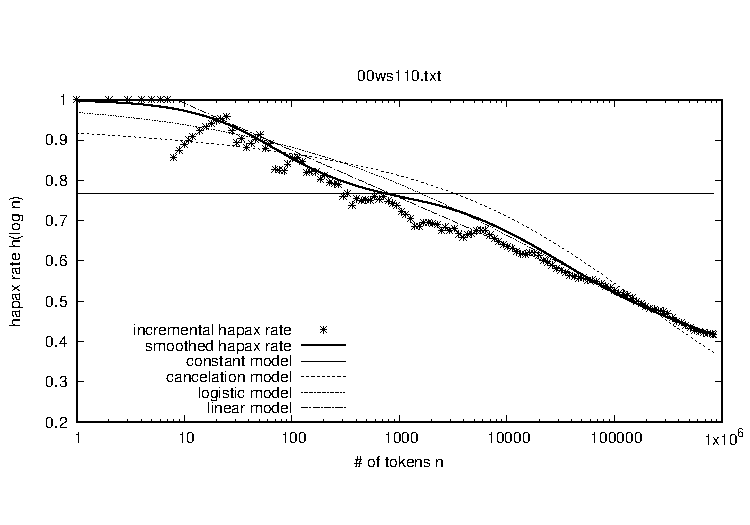
\includegraphics[width=0.8\columnwidth]{output/herdan/00ws110_27/token_ratio.pdf}
  \\[-3em]
  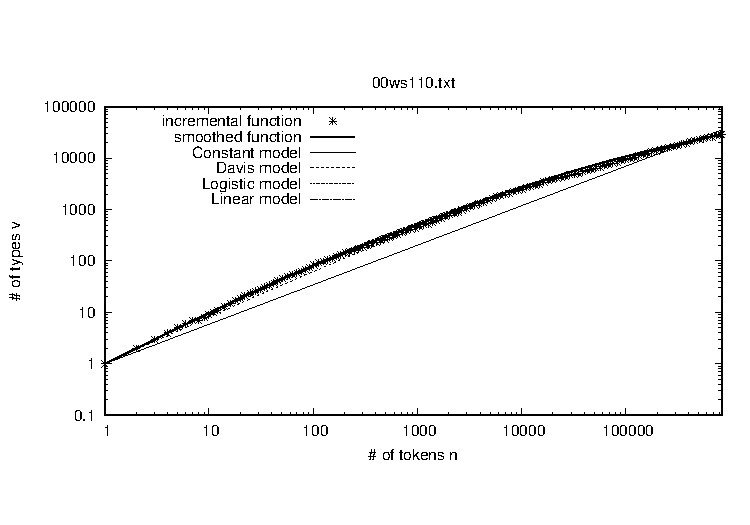
\includegraphics[width=0.8\columnwidth]{output/herdan/00ws110_27/token_type.pdf}
  \\[-3em]
  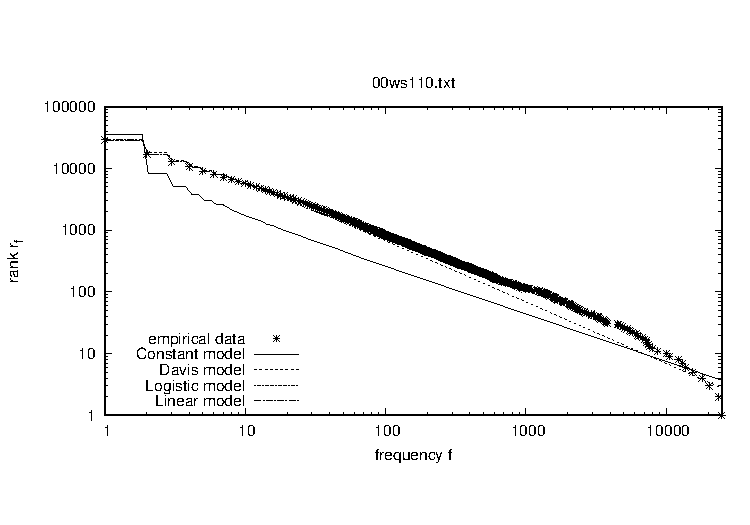
\includegraphics[width=0.8\columnwidth]{output/herdan/00ws110_27/frequency_rank.pdf}
  \vspace{-2em}
  \caption{W. Shakespeare, \emph{First Folio/35 Plays}.\label{fig00ws110F}}
\end{figure}

\begin{figure}[p]
  \centering
  \vspace{-2em}
  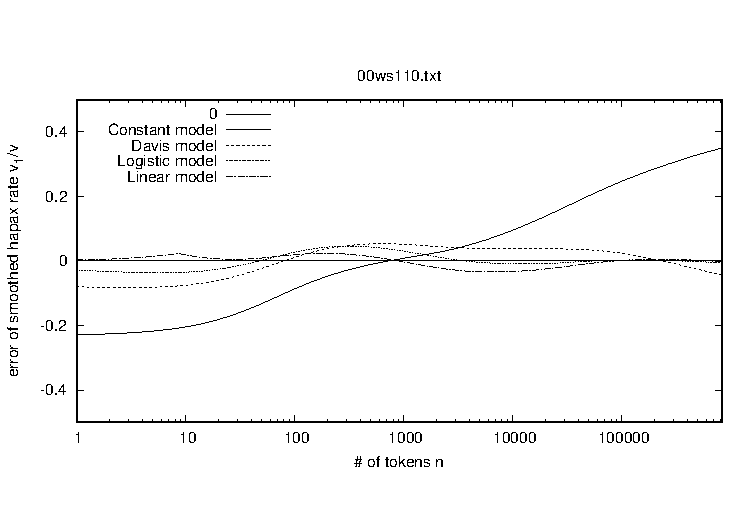
\includegraphics[width=0.8\columnwidth]{output/herdan/00ws110_27/token_ratio_residual.pdf}
  \\[-3em]
  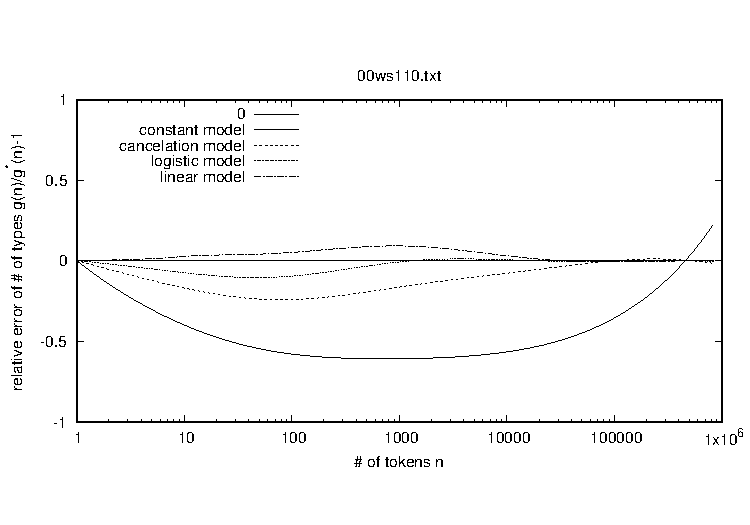
\includegraphics[width=0.8\columnwidth]{output/herdan/00ws110_27/token_residual.pdf}
  \\[-3em]
  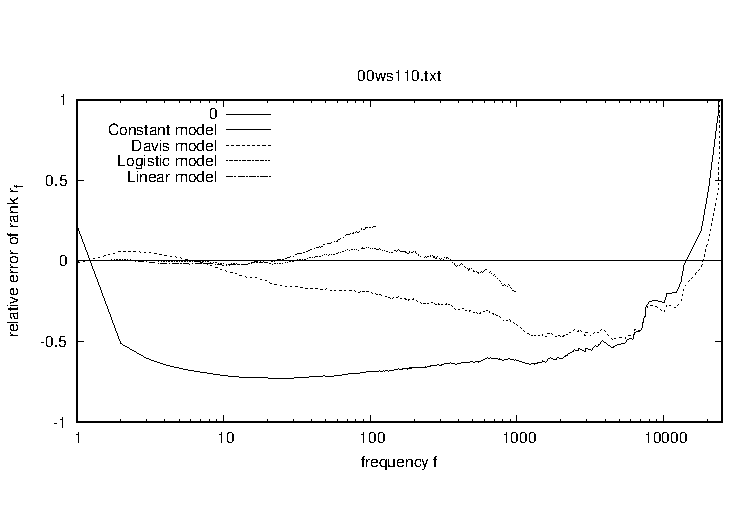
\includegraphics[width=0.8\columnwidth]{output/herdan/00ws110_27/frequency_residual.pdf}
  \vspace{-2em}
  \caption{W. Shakespeare, \emph{First Folio/35 Plays}.\label{fig00ws110R}}
\end{figure}

%%%%%%%%%%%

\begin{figure}[p]
  \centering
  \vspace{-2em}
  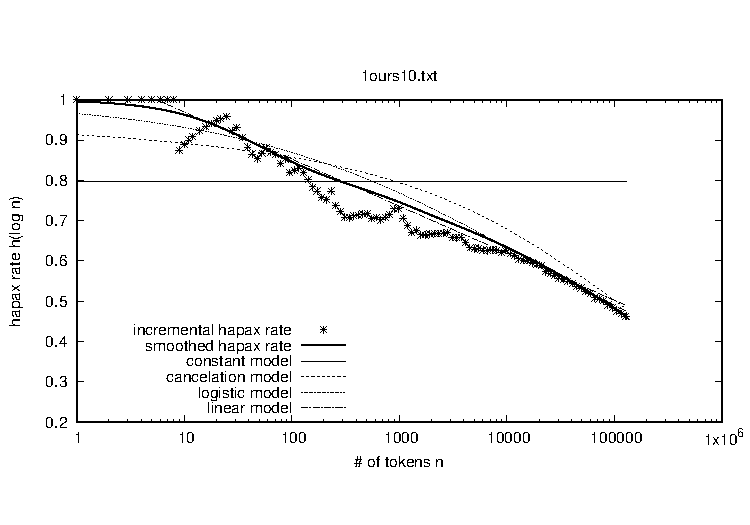
\includegraphics[width=0.8\columnwidth]{output/herdan/1ours10_27/token_ratio.pdf}
  \\[-3em]
  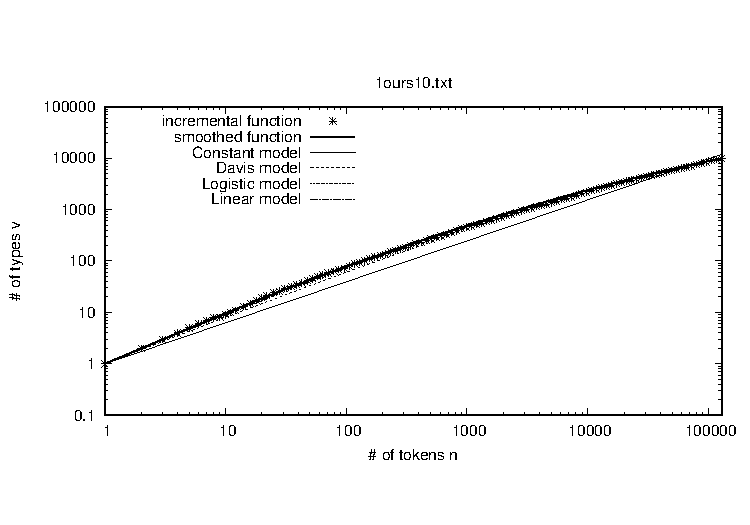
\includegraphics[width=0.8\columnwidth]{output/herdan/1ours10_27/token_type.pdf}
  \\[-3em]
  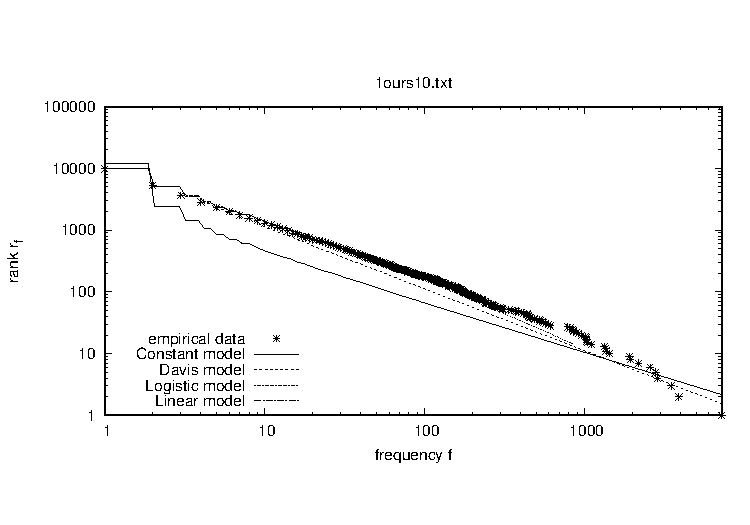
\includegraphics[width=0.8\columnwidth]{output/herdan/1ours10_27/frequency_rank.pdf}
  \vspace{-2em}
  \caption{W. Cather, \emph{One of Ours}.\label{fig1ours10F}}
\end{figure}

\begin{figure}[p]
  \centering
  \vspace{-2em}
  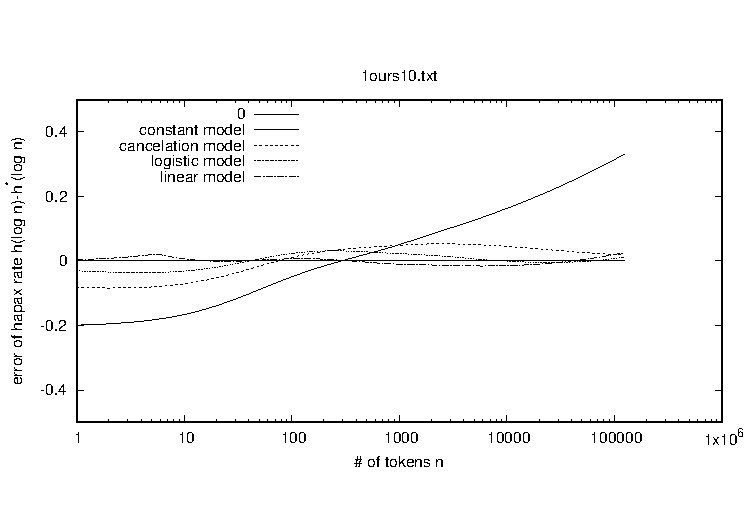
\includegraphics[width=0.8\columnwidth]{output/herdan/1ours10_27/token_ratio_residual.pdf}
  \\[-3em]
  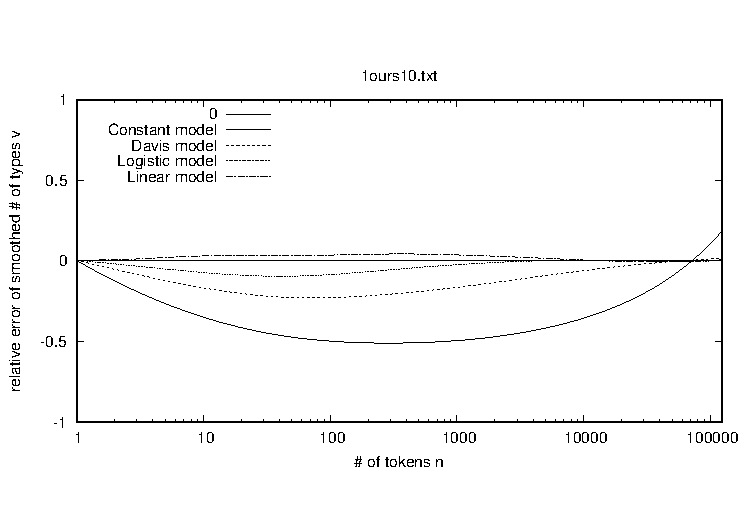
\includegraphics[width=0.8\columnwidth]{output/herdan/1ours10_27/token_residual.pdf}
  \\[-3em]
  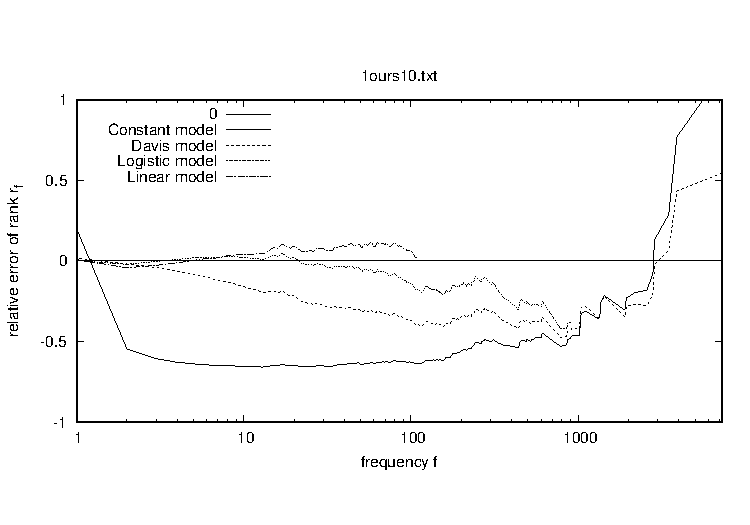
\includegraphics[width=0.8\columnwidth]{output/herdan/1ours10_27/frequency_residual.pdf}
  \vspace{-2em}
  \caption{W. Cather, \emph{One of Ours}.\label{fig1ours10R}}
\end{figure}

%%%%%%%%%%%

\begin{figure}[p]
  \centering
  \vspace{-2em}
  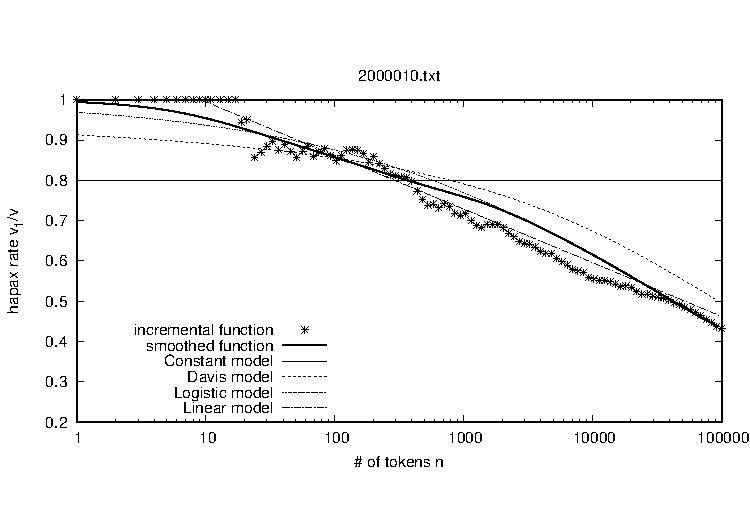
\includegraphics[width=0.8\columnwidth]{output/herdan/2000010_27/token_ratio.pdf}
  \\[-3em]
  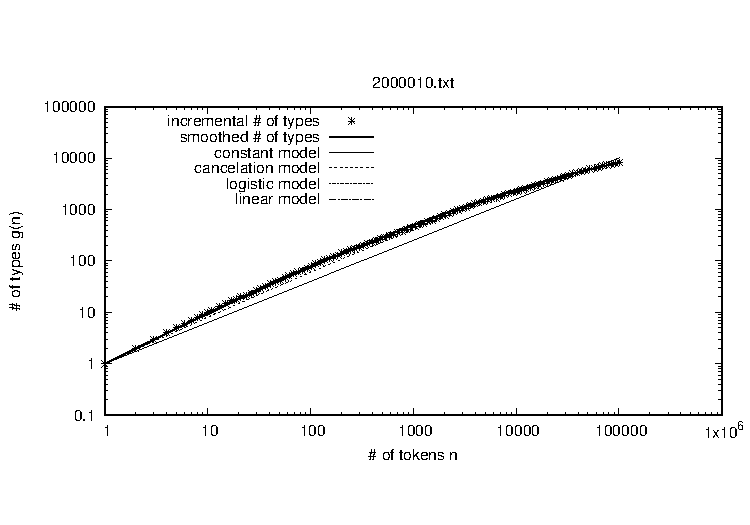
\includegraphics[width=0.8\columnwidth]{output/herdan/2000010_27/token_type.pdf}
  \\[-3em]
  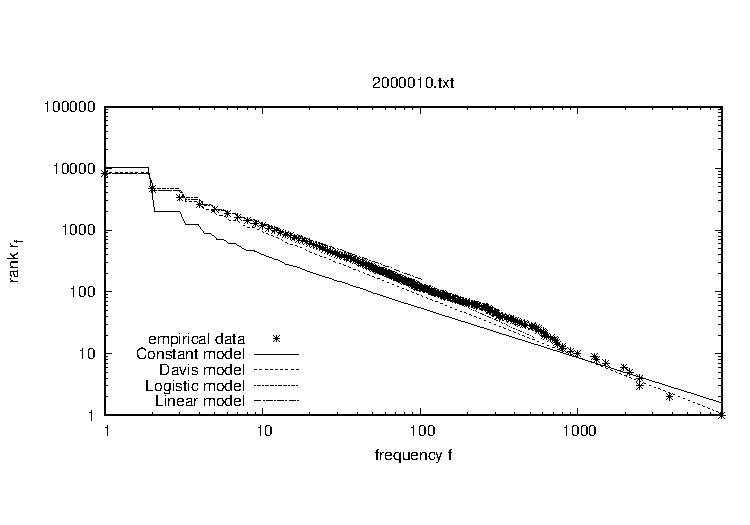
\includegraphics[width=0.8\columnwidth]{output/herdan/2000010_27/frequency_rank.pdf}
  \vspace{-2em}
  \caption{J. Verne, \emph{20,000 Leagues under the Sea}.\label{fig2000010F}}
\end{figure}

\begin{figure}[p]
  \centering
  \vspace{-2em}
  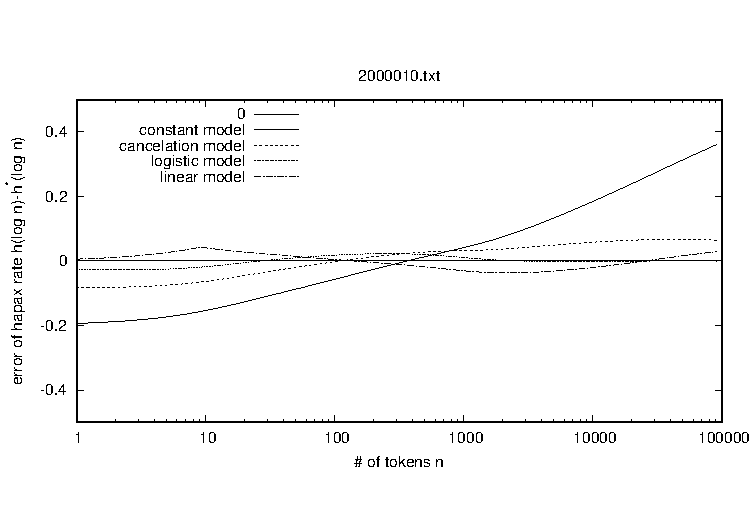
\includegraphics[width=0.8\columnwidth]{output/herdan/2000010_27/token_ratio_residual.pdf}
  \\[-3em]
  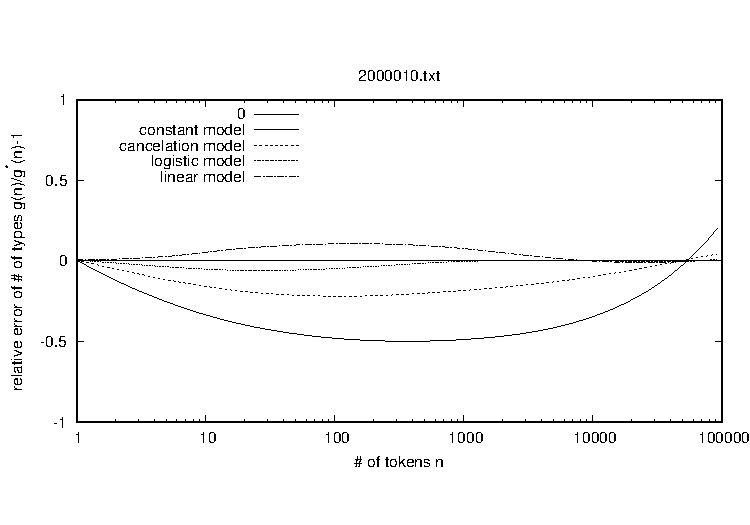
\includegraphics[width=0.8\columnwidth]{output/herdan/2000010_27/token_residual.pdf}
  \\[-3em]
  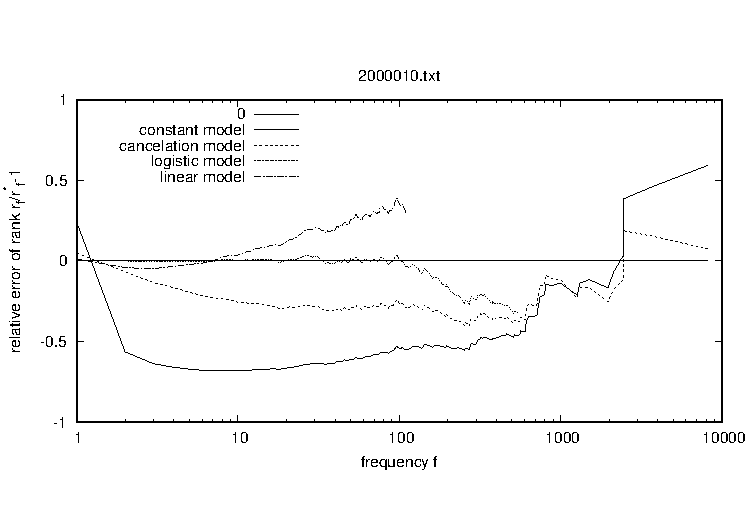
\includegraphics[width=0.8\columnwidth]{output/herdan/2000010_27/frequency_residual.pdf}
  \vspace{-2em}
  \caption{J. Verne, \emph{20,000 Leagues under the Sea}.\label{fig2000010R}}
\end{figure}

%%%%%%%%%%%

\begin{figure}[p]
  \centering
  \vspace{-2em}
  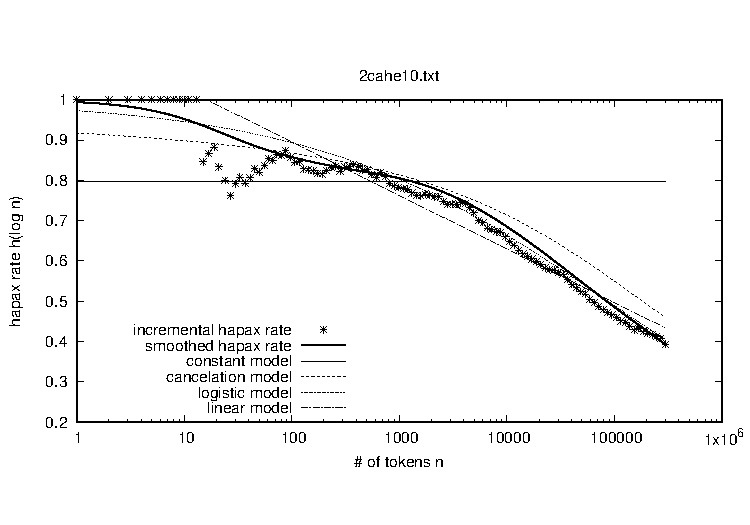
\includegraphics[width=0.8\columnwidth]{output/herdan/2cahe10_27/token_ratio.pdf}
  \\[-3em]
  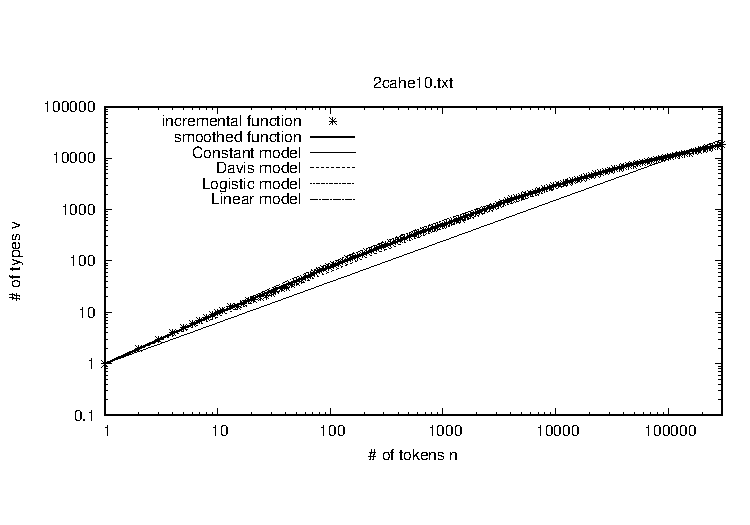
\includegraphics[width=0.8\columnwidth]{output/herdan/2cahe10_27/token_type.pdf}
  \\[-3em]
  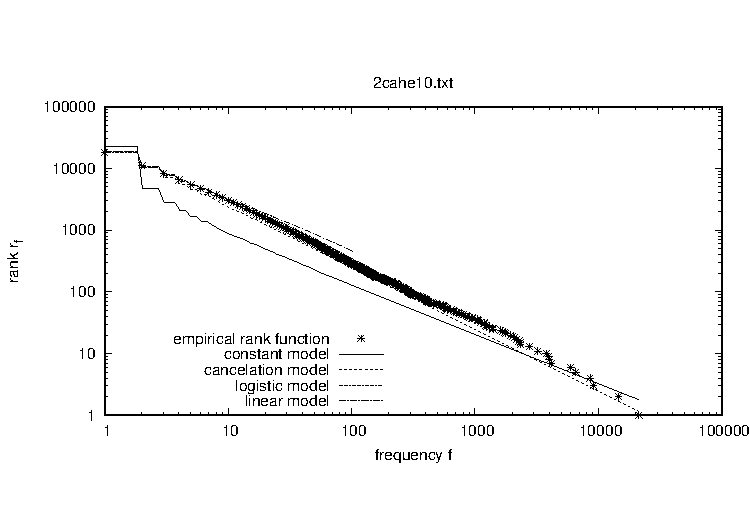
\includegraphics[width=0.8\columnwidth]{output/herdan/2cahe10_27/frequency_rank.pdf}
  \vspace{-2em}
  \caption{T. Macaulay, \emph{Critical \& Historical
      Essays}.\label{fig2cahe10F}}
\end{figure}

\begin{figure}[p]
  \centering
  \vspace{-2em}
  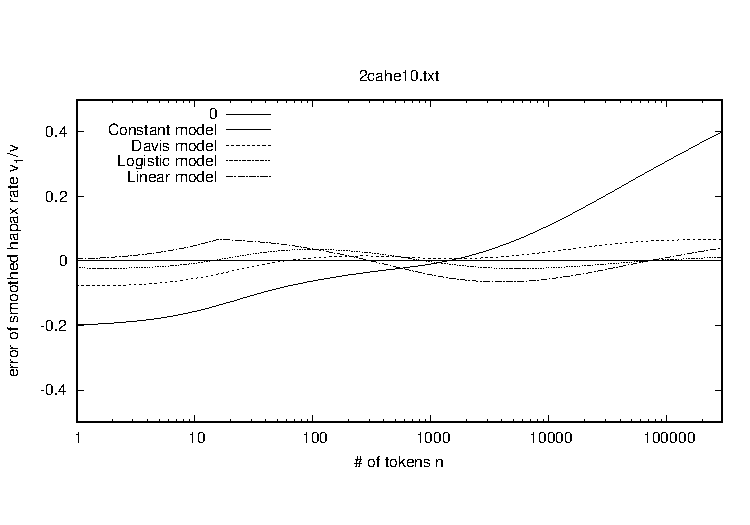
\includegraphics[width=0.8\columnwidth]{output/herdan/2cahe10_27/token_ratio_residual.pdf}
  \\[-3em]
  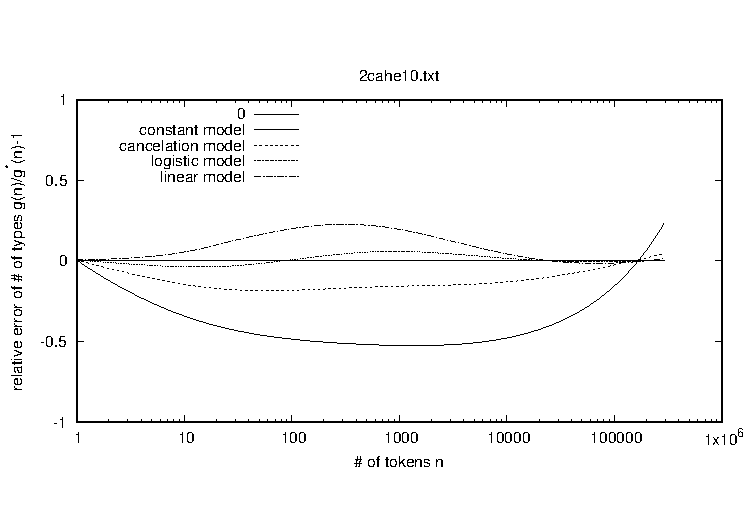
\includegraphics[width=0.8\columnwidth]{output/herdan/2cahe10_27/token_residual.pdf}
  \\[-3em]
  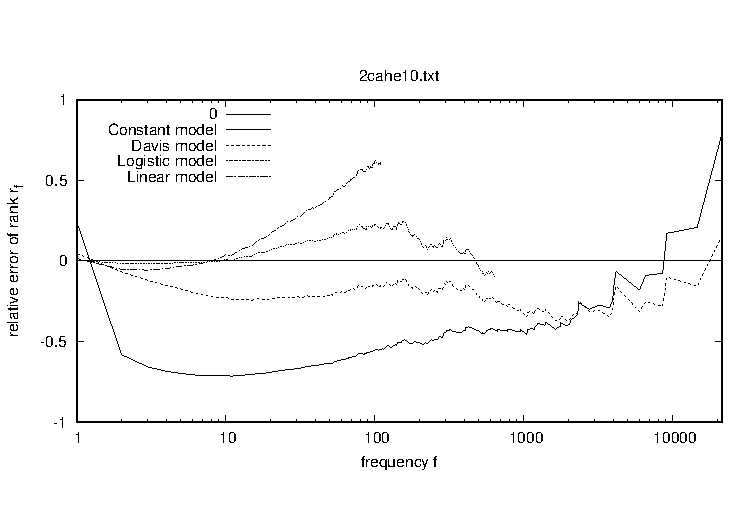
\includegraphics[width=0.8\columnwidth]{output/herdan/2cahe10_27/frequency_residual.pdf}
  \vspace{-2em}
  \caption{T. Macaulay, \emph{Critical \& Historical
      Essays}.\label{fig2cahe10R}}
\end{figure}

%%%%%%%%%%%

\begin{figure}[p]
  \centering
  \vspace{-2em}
  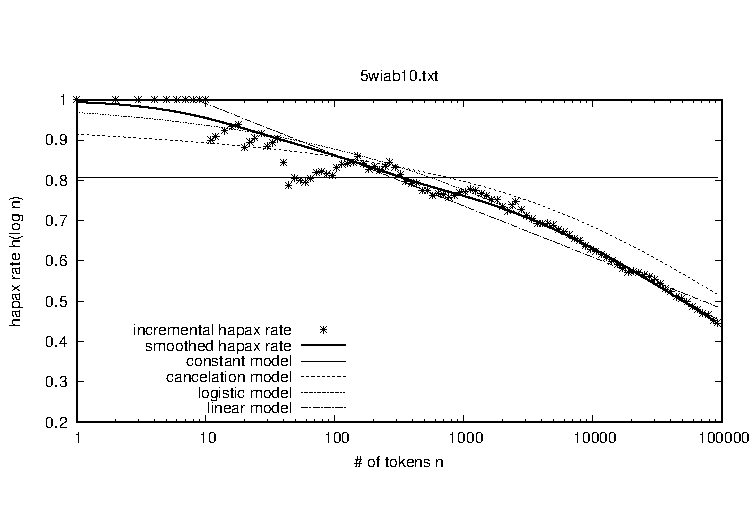
\includegraphics[width=0.8\columnwidth]{output/herdan/5wiab10_27/token_ratio.pdf}
  \\[-3em]
  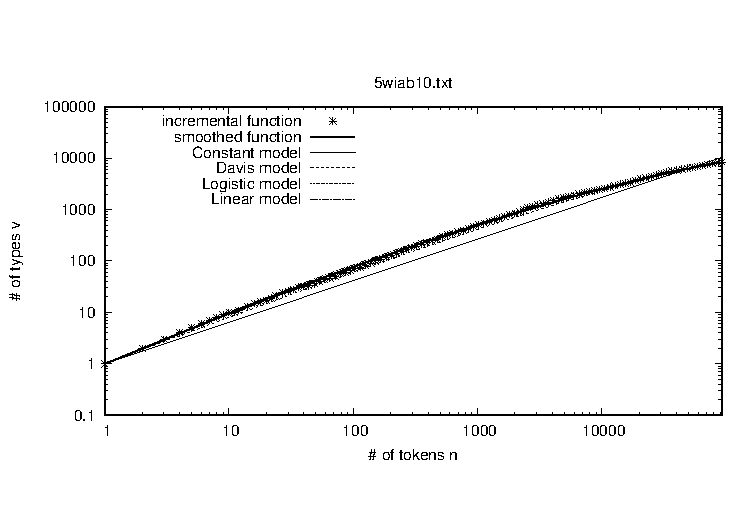
\includegraphics[width=0.8\columnwidth]{output/herdan/5wiab10_27/token_type.pdf}
  \\[-3em]
  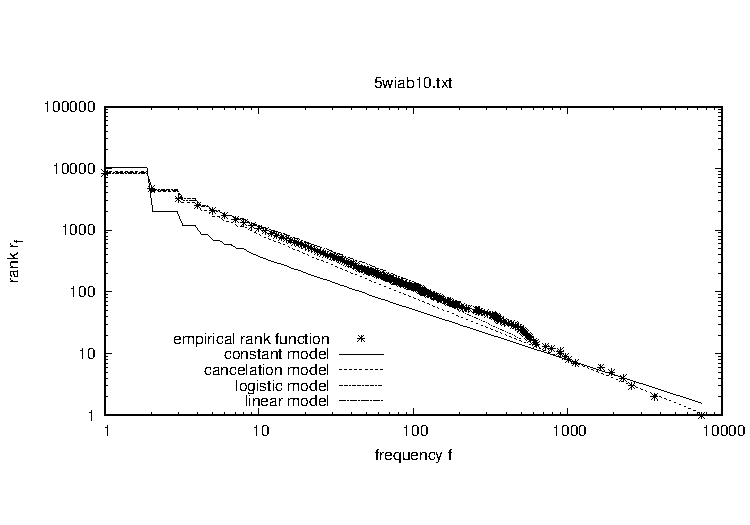
\includegraphics[width=0.8\columnwidth]{output/herdan/5wiab10_27/frequency_rank.pdf}
  \vspace{-2em}
  \caption{J. Verne, \emph{Five Weeks in a Balloon}.\label{fig5wiab10F}}
\end{figure}

\begin{figure}[p]
  \centering
  \vspace{-2em}
  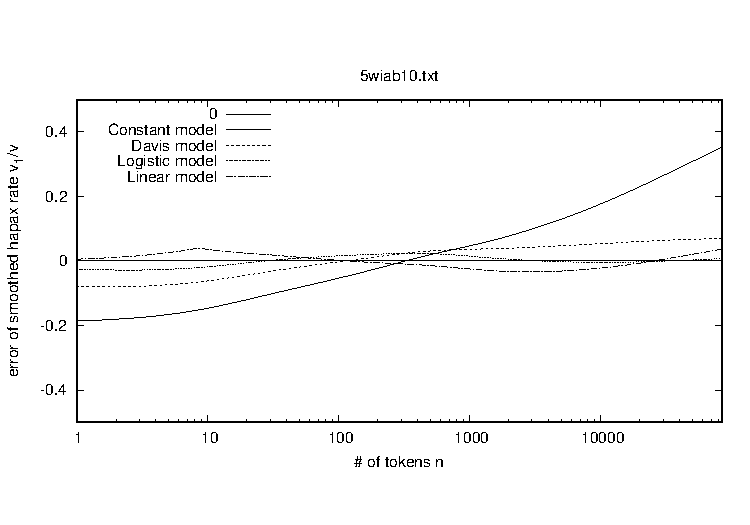
\includegraphics[width=0.8\columnwidth]{output/herdan/5wiab10_27/token_ratio_residual.pdf}
  \\[-3em]
  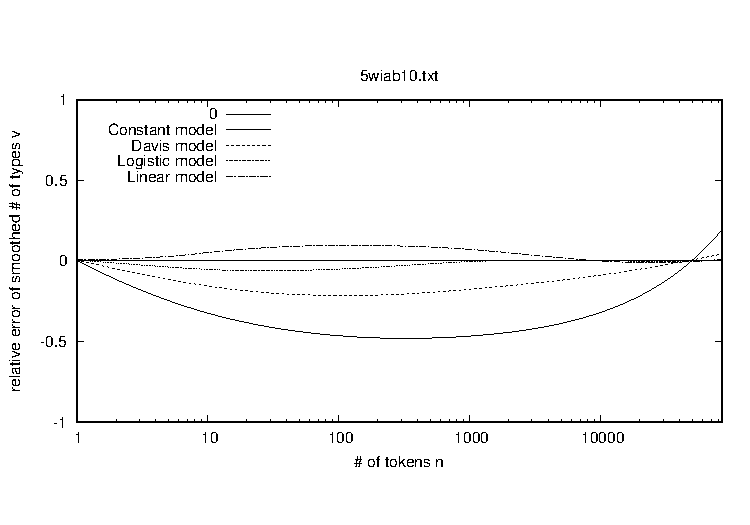
\includegraphics[width=0.8\columnwidth]{output/herdan/5wiab10_27/token_residual.pdf}
  \\[-3em]
  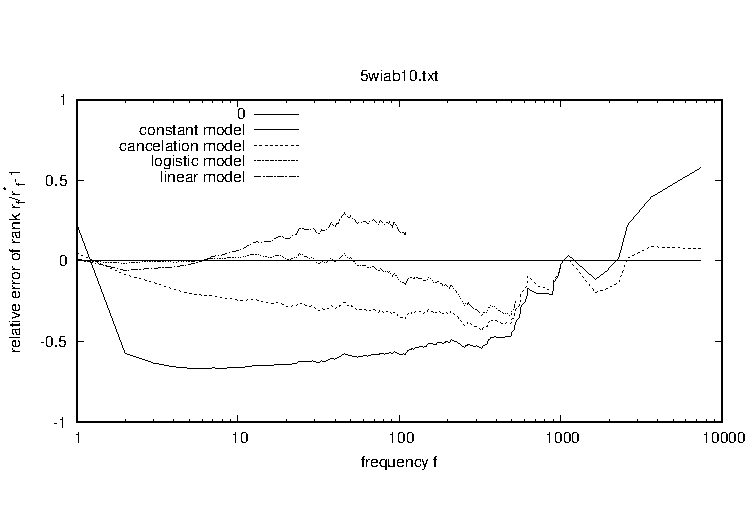
\includegraphics[width=0.8\columnwidth]{output/herdan/5wiab10_27/frequency_residual.pdf}
  \vspace{-2em}
  \caption{J. Verne, \emph{Five Weeks in a Balloon}.\label{fig5wiab10R}}
\end{figure}

%%%%%%%%%%%

\begin{figure}[p]
  \centering
  \vspace{-2em}
  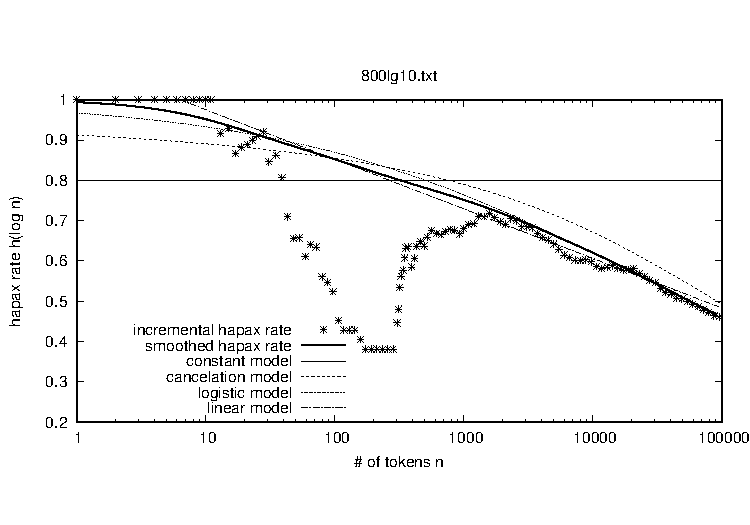
\includegraphics[width=0.8\columnwidth]{output/herdan/800lg10_27/token_ratio.pdf}
  \\[-3em]
  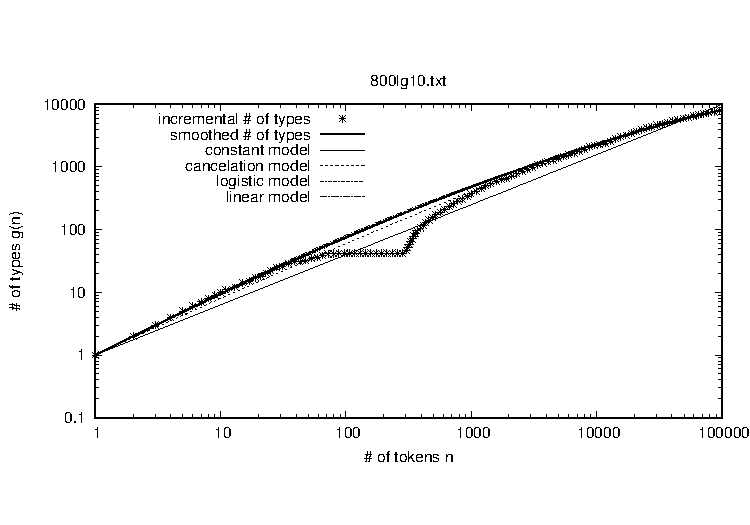
\includegraphics[width=0.8\columnwidth]{output/herdan/800lg10_27/token_type.pdf}
  \\[-3em]
  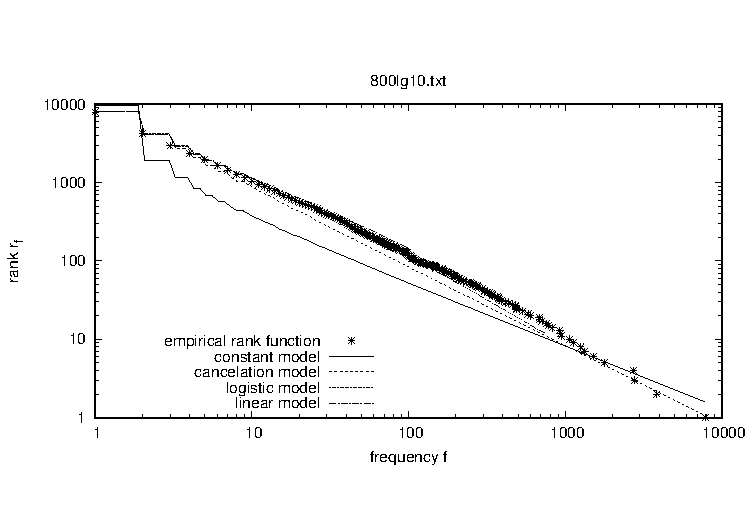
\includegraphics[width=0.8\columnwidth]{output/herdan/800lg10_27/frequency_rank.pdf}
  \vspace{-2em}
  \caption{J. Verne, \emph{Eight Hundred Leagues on the
      Amazon}.\label{fig800lg10F}}
\end{figure}

\begin{figure}[p]
  \centering
  \vspace{-2em}
  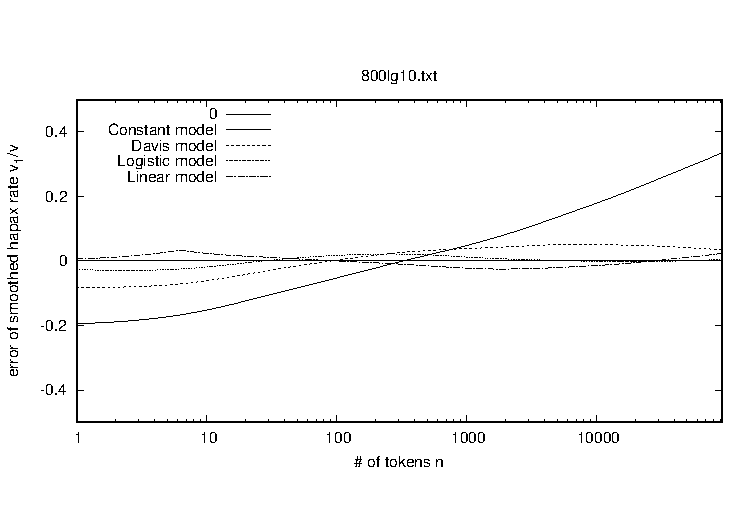
\includegraphics[width=0.8\columnwidth]{output/herdan/800lg10_27/token_ratio_residual.pdf}
  \\[-3em]
  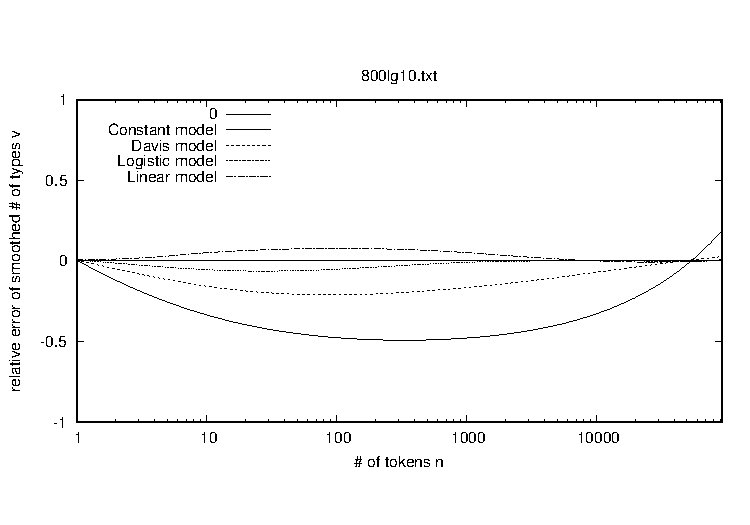
\includegraphics[width=0.8\columnwidth]{output/herdan/800lg10_27/token_residual.pdf}
  \\[-3em]
  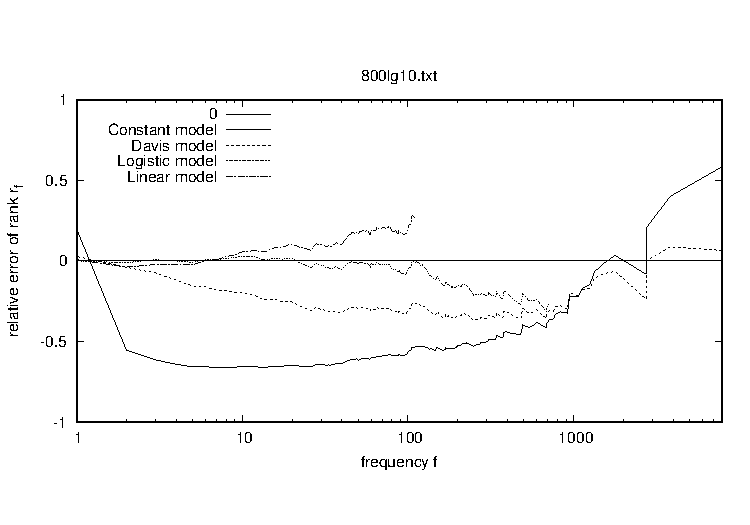
\includegraphics[width=0.8\columnwidth]{output/herdan/800lg10_27/frequency_residual.pdf}
  \vspace{-2em}
  \caption{J. Verne, \emph{Eight Hundred Leagues on the
      Amazon}.\label{fig800lg10R}}
\end{figure}

%%%%%%%%%%%

\begin{figure}[p]
  \centering
  \vspace{-2em}
  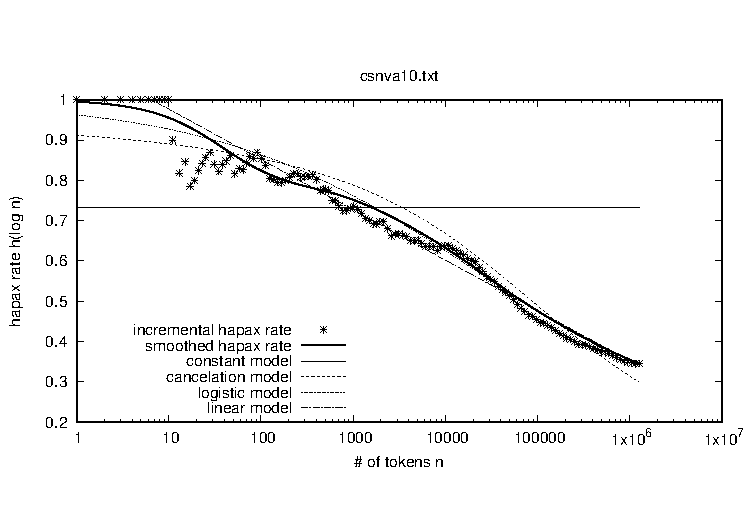
\includegraphics[width=0.8\columnwidth]{output/herdan/csnva10_27/token_ratio.pdf}
  \\[-3em]
  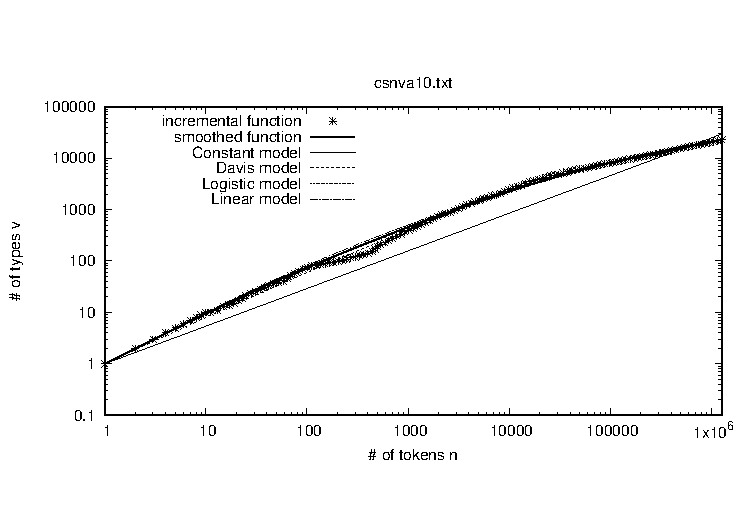
\includegraphics[width=0.8\columnwidth]{output/herdan/csnva10_27/token_type.pdf}
  \\[-3em]
  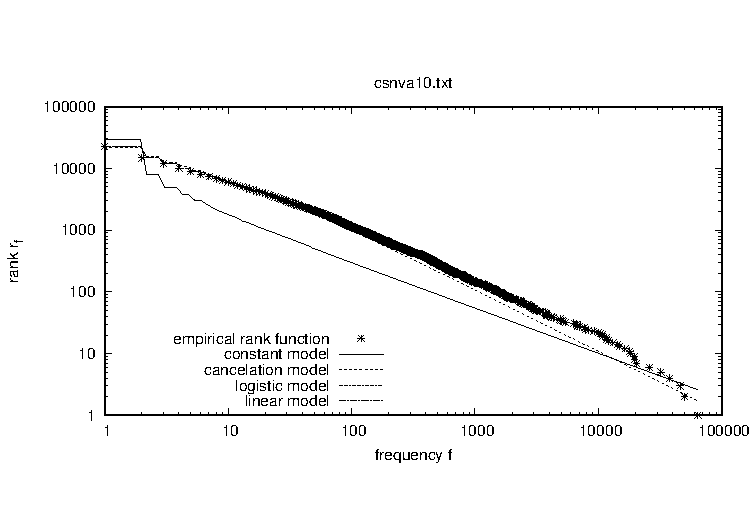
\includegraphics[width=0.8\columnwidth]{output/herdan/csnva10_27/frequency_rank.pdf}
  \vspace{-2em}
  \caption{J. Casanova, \emph{The Complete Memoirs}.\label{figcsnva10F}}
\end{figure}

\begin{figure}[p]
  \centering
  \vspace{-2em}
  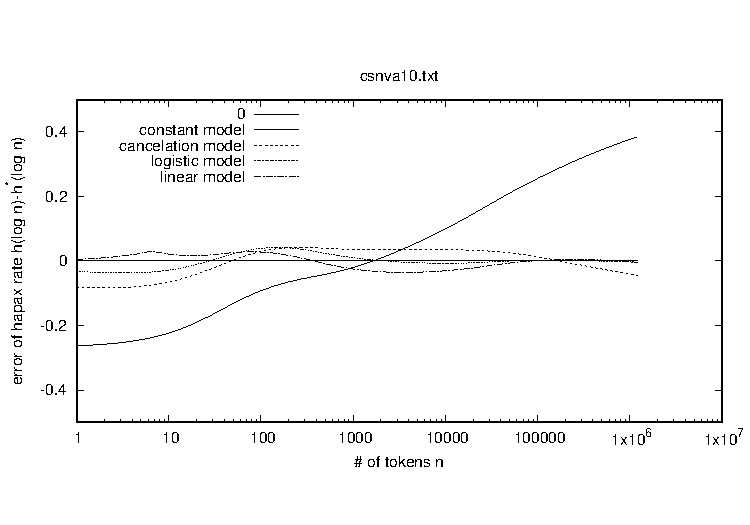
\includegraphics[width=0.8\columnwidth]{output/herdan/csnva10_27/token_ratio_residual.pdf}
  \\[-3em]
  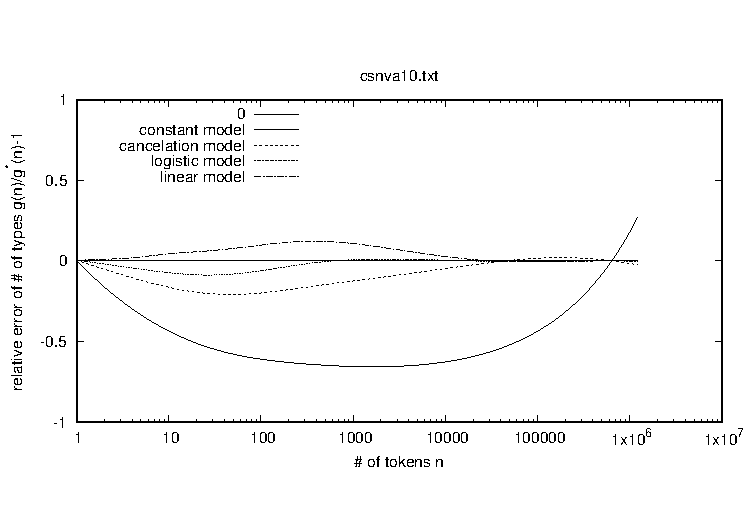
\includegraphics[width=0.8\columnwidth]{output/herdan/csnva10_27/token_residual.pdf}
  \\[-3em]
  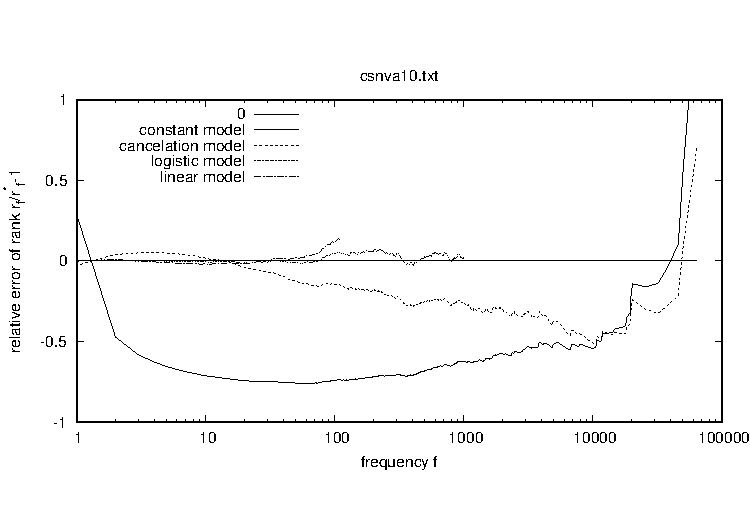
\includegraphics[width=0.8\columnwidth]{output/herdan/csnva10_27/frequency_residual.pdf}
  \vspace{-2em}
  \caption{J. Casanova, \emph{The Complete Memoirs}.\label{figcsnva10R}}
\end{figure}

%%%%%%%%%%%

\begin{figure}[p]
  \centering
  \vspace{-2em}
  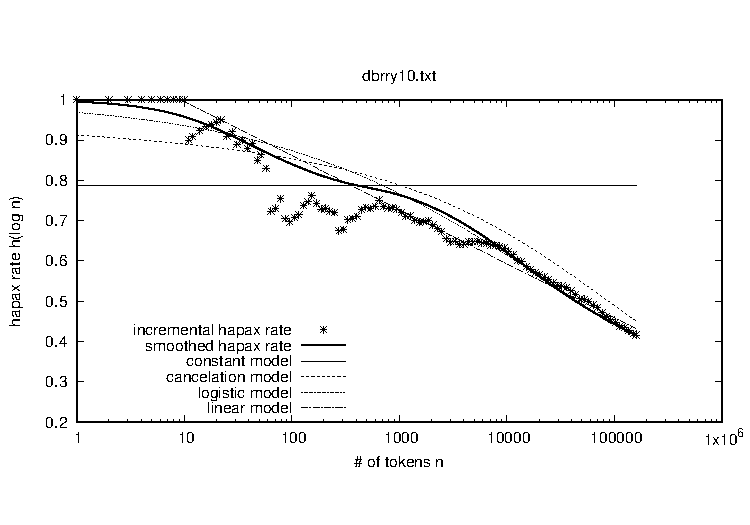
\includegraphics[width=0.8\columnwidth]{output/herdan/dbrry10_27/token_ratio.pdf}
  \\[-3em]
  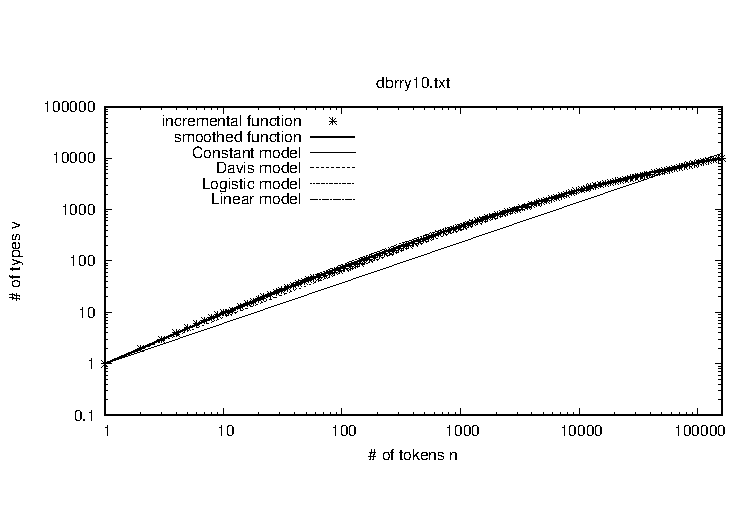
\includegraphics[width=0.8\columnwidth]{output/herdan/dbrry10_27/token_type.pdf}
  \\[-3em]
  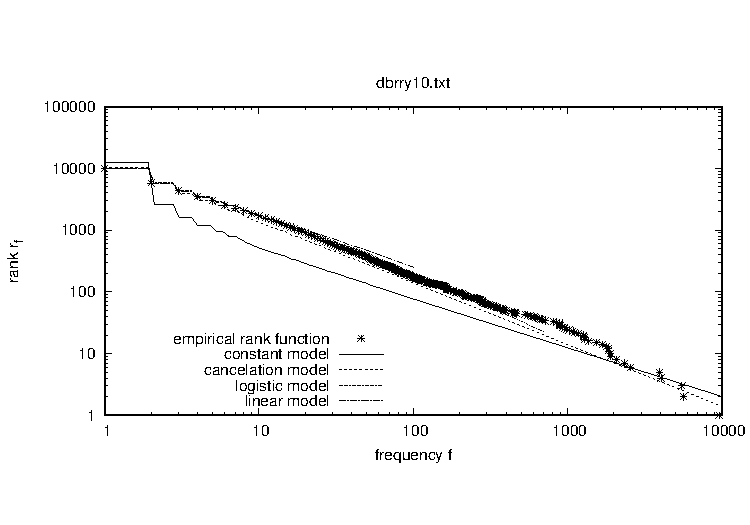
\includegraphics[width=0.8\columnwidth]{output/herdan/dbrry10_27/frequency_rank.pdf}
  \vspace{-2em}
  \caption{Comtesse du Barry, \emph{Memoirs}.\label{figdbrry10F}}
\end{figure}

\begin{figure}[p]
  \centering
  \vspace{-2em}
  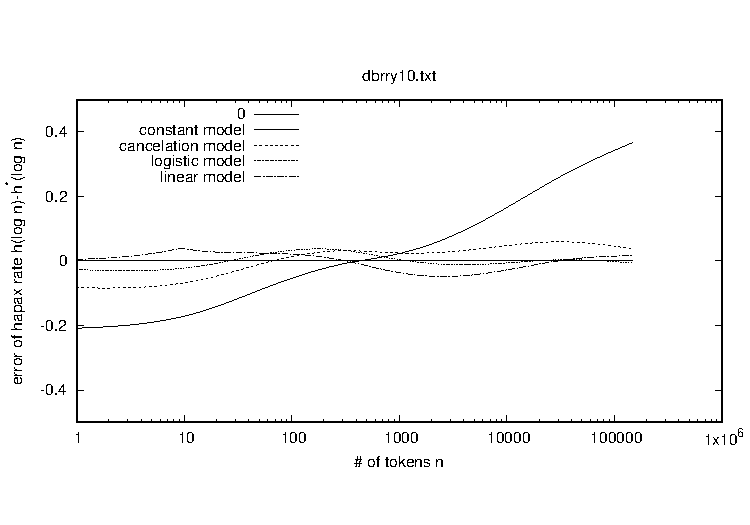
\includegraphics[width=0.8\columnwidth]{output/herdan/dbrry10_27/token_ratio_residual.pdf}
  \\[-3em]
  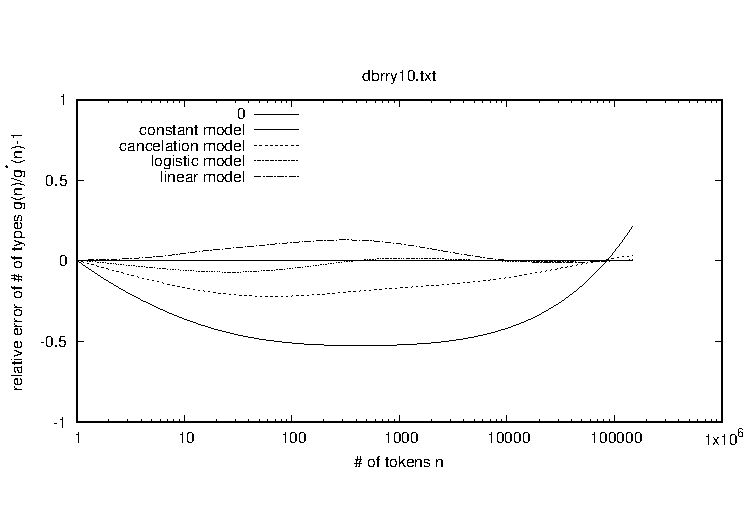
\includegraphics[width=0.8\columnwidth]{output/herdan/dbrry10_27/token_residual.pdf}
  \\[-3em]
  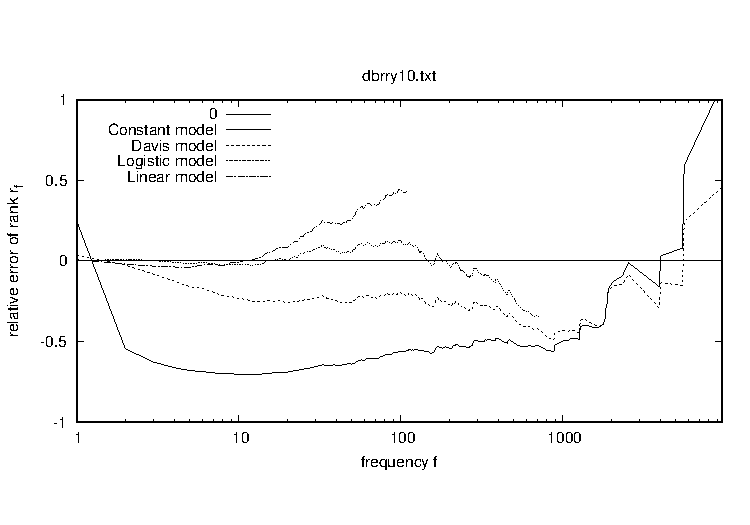
\includegraphics[width=0.8\columnwidth]{output/herdan/dbrry10_27/frequency_residual.pdf}
  \vspace{-2em}
  \caption{Comtesse du Barry, \emph{Memoirs}.\label{figdbrry10R}}
\end{figure}

%%%%%%%%%%%

\begin{figure}[p]
  \centering
  \vspace{-2em}
  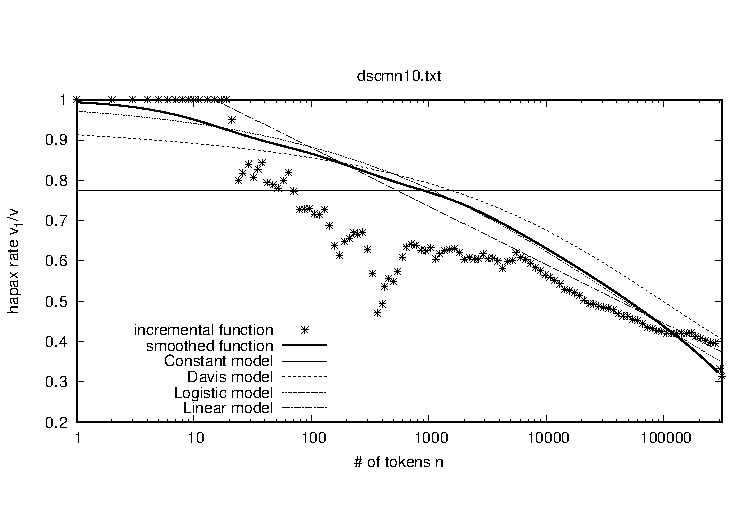
\includegraphics[width=0.8\columnwidth]{output/herdan/dscmn10_27/token_ratio.pdf}
  \\[-3em]
  \includegraphics[width=0.8\columnwidth]{output/herdan/dscmn10_27/token_type.pdf}
  \\[-3em]
  \includegraphics[width=0.8\columnwidth]{output/herdan/dscmn10_27/frequency_rank.pdf}
  \vspace{-2em}
  \caption{C. Darwin, \emph{The Descent of Man}.\label{figdscmn10F}}
\end{figure}

\begin{figure}[p]
  \centering
  \vspace{-2em}
  \includegraphics[width=0.8\columnwidth]{output/herdan/dscmn10_27/token_ratio_residual.pdf}
  \\[-3em]
  \includegraphics[width=0.8\columnwidth]{output/herdan/dscmn10_27/token_residual.pdf}
  \\[-3em]
  \includegraphics[width=0.8\columnwidth]{output/herdan/dscmn10_27/frequency_residual.pdf}
  \vspace{-2em}
  \caption{C. Darwin, \emph{The Descent of Man}.\label{figdscmn10R}}
\end{figure}

%%%%%%%%%%%

\begin{figure}[p]
  \centering
  \vspace{-2em}
  \includegraphics[width=0.8\columnwidth]{output/herdan/gltrv10_27/token_ratio.pdf}
  \\[-3em]
  \includegraphics[width=0.8\columnwidth]{output/herdan/gltrv10_27/token_type.pdf}
  \\[-3em]
  \includegraphics[width=0.8\columnwidth]{output/herdan/gltrv10_27/frequency_rank.pdf}
  \vspace{-2em}
  \caption{J. Swift, \emph{Gulliver’s Travels}.\label{figgltrv10F}}
\end{figure}

\begin{figure}[p]
  \centering
  \vspace{-2em}
  \includegraphics[width=0.8\columnwidth]{output/herdan/gltrv10_27/token_ratio_residual.pdf}
  \\[-3em]
  \includegraphics[width=0.8\columnwidth]{output/herdan/gltrv10_27/token_residual.pdf}
  \\[-3em]
  \includegraphics[width=0.8\columnwidth]{output/herdan/gltrv10_27/frequency_residual.pdf}
  \vspace{-2em}
  \caption{J. Swift, \emph{Gulliver’s Travels}.\label{figgltrv10R}}
\end{figure}

%%%%%%%%%%%

\begin{figure}[p]
  \centering
  \vspace{-2em}
  \includegraphics[width=0.8\columnwidth]{output/herdan/milnd10_27/token_ratio.pdf}
  \\[-3em]
  \includegraphics[width=0.8\columnwidth]{output/herdan/milnd10_27/token_type.pdf}
  \\[-3em]
  \includegraphics[width=0.8\columnwidth]{output/herdan/milnd10_27/frequency_rank.pdf}
  \vspace{-2em}
  \caption{J. Verne, \emph{The Mysterious Island}.\label{figmilnd10F}}
\end{figure}

\begin{figure}[p]
  \centering
  \vspace{-2em}
  \includegraphics[width=0.8\columnwidth]{output/herdan/milnd10_27/token_ratio_residual.pdf}
  \\[-3em]
  \includegraphics[width=0.8\columnwidth]{output/herdan/milnd10_27/token_residual.pdf}
  \\[-3em]
  \includegraphics[width=0.8\columnwidth]{output/herdan/milnd10_27/frequency_residual.pdf}
  \vspace{-2em}
  \caption{J. Verne, \emph{The Mysterious Island}.\label{figmilnd10R}}
\end{figure}

%%%%%%%%%%%

\begin{figure}[p]
  \centering
  \vspace{-2em}
  \includegraphics[width=0.8\columnwidth]{output/herdan/mt7bg10_27/token_ratio.pdf}
  \\[-3em]
  \includegraphics[width=0.8\columnwidth]{output/herdan/mt7bg10_27/token_type.pdf}
  \\[-3em]
  \includegraphics[width=0.8\columnwidth]{output/herdan/mt7bg10_27/frequency_rank.pdf}
  \vspace{-2em}
  \caption{A. Paine, \emph{Mark Twain, A Biography}.\label{figmt7bg10F}}
\end{figure}

\begin{figure}[p]
  \centering
  \vspace{-2em}
  \includegraphics[width=0.8\columnwidth]{output/herdan/mt7bg10_27/token_ratio_residual.pdf}
  \\[-3em]
  \includegraphics[width=0.8\columnwidth]{output/herdan/mt7bg10_27/token_residual.pdf}
  \\[-3em]
  \includegraphics[width=0.8\columnwidth]{output/herdan/mt7bg10_27/frequency_residual.pdf}
  \vspace{-2em}
  \caption{A. Paine, \emph{Mark Twain, A Biography}.\label{figmt7bg10R}}
\end{figure}

%%%%%%%%%%%

\begin{figure}[p]
  \centering
  \vspace{-2em}
  \includegraphics[width=0.8\columnwidth]{output/herdan/stlla10_27/token_ratio.pdf}
  \\[-3em]
  \includegraphics[width=0.8\columnwidth]{output/herdan/stlla10_27/token_type.pdf}
  \\[-3em]
  \includegraphics[width=0.8\columnwidth]{output/herdan/stlla10_27/frequency_rank.pdf}
  \vspace{-2em}
  \caption{J. Swift, \emph{The Journal to Stella}.\label{figstlla10F}}
\end{figure}

\begin{figure}[p]
  \centering
  \vspace{-2em}
  \includegraphics[width=0.8\columnwidth]{output/herdan/stlla10_27/token_ratio_residual.pdf}
  \\[-3em]
  \includegraphics[width=0.8\columnwidth]{output/herdan/stlla10_27/token_residual.pdf}
  \\[-3em]
  \includegraphics[width=0.8\columnwidth]{output/herdan/stlla10_27/frequency_residual.pdf}
  \vspace{-2em}
  \caption{J. Swift, \emph{The Journal to Stella}.\label{figstlla10R}}
\end{figure}

%%%%%%%%%%%

\begin{figure}[p]
  \centering
  \vspace{-2em}
  \includegraphics[width=0.8\columnwidth]{output/herdan/wmcry10_27/token_ratio.pdf}
  \\[-3em]
  \includegraphics[width=0.8\columnwidth]{output/herdan/wmcry10_27/token_type.pdf}
  \\[-3em]
  \includegraphics[width=0.8\columnwidth]{output/herdan/wmcry10_27/frequency_rank.pdf}
  \vspace{-2em}
  \caption{G. Smith, \emph{Life of William Carey}.\label{figwmcry10F}}
\end{figure}

\begin{figure}[p]
  \centering
  \vspace{-2em}
  \includegraphics[width=0.8\columnwidth]{output/herdan/wmcry10_27/token_ratio_residual.pdf}
  \\[-3em]
  \includegraphics[width=0.8\columnwidth]{output/herdan/wmcry10_27/token_residual.pdf}
  \\[-3em]
  \includegraphics[width=0.8\columnwidth]{output/herdan/wmcry10_27/frequency_residual.pdf}
  \vspace{-2em}
  \caption{G. Smith, \emph{Life of William Carey}.\label{figwmcry10R}}
\end{figure}


%\setlength{\bibsep}{2pt}
\bibliography{0-publishers-full,0-journals-full,books,ql,nlp,ai,mine}


\end{document}

